\section{Interfejs użytkownika}
\label{sec:interfejs_uzytkownika}

Ostatnim elementem aplikacji,
łączącym wszystkie funkcje w~całość oraz umożliwiającym użytkownikowi interakcję z~programem,
jest interfejs użytkownika (ang. \textit{User Interface}, UI).
Ostateczny widok okna aplikacji podczas działania programu pokazano na rysunku~\ref{fig:ui_final}.

\begin{figure}[H]
    \centering
    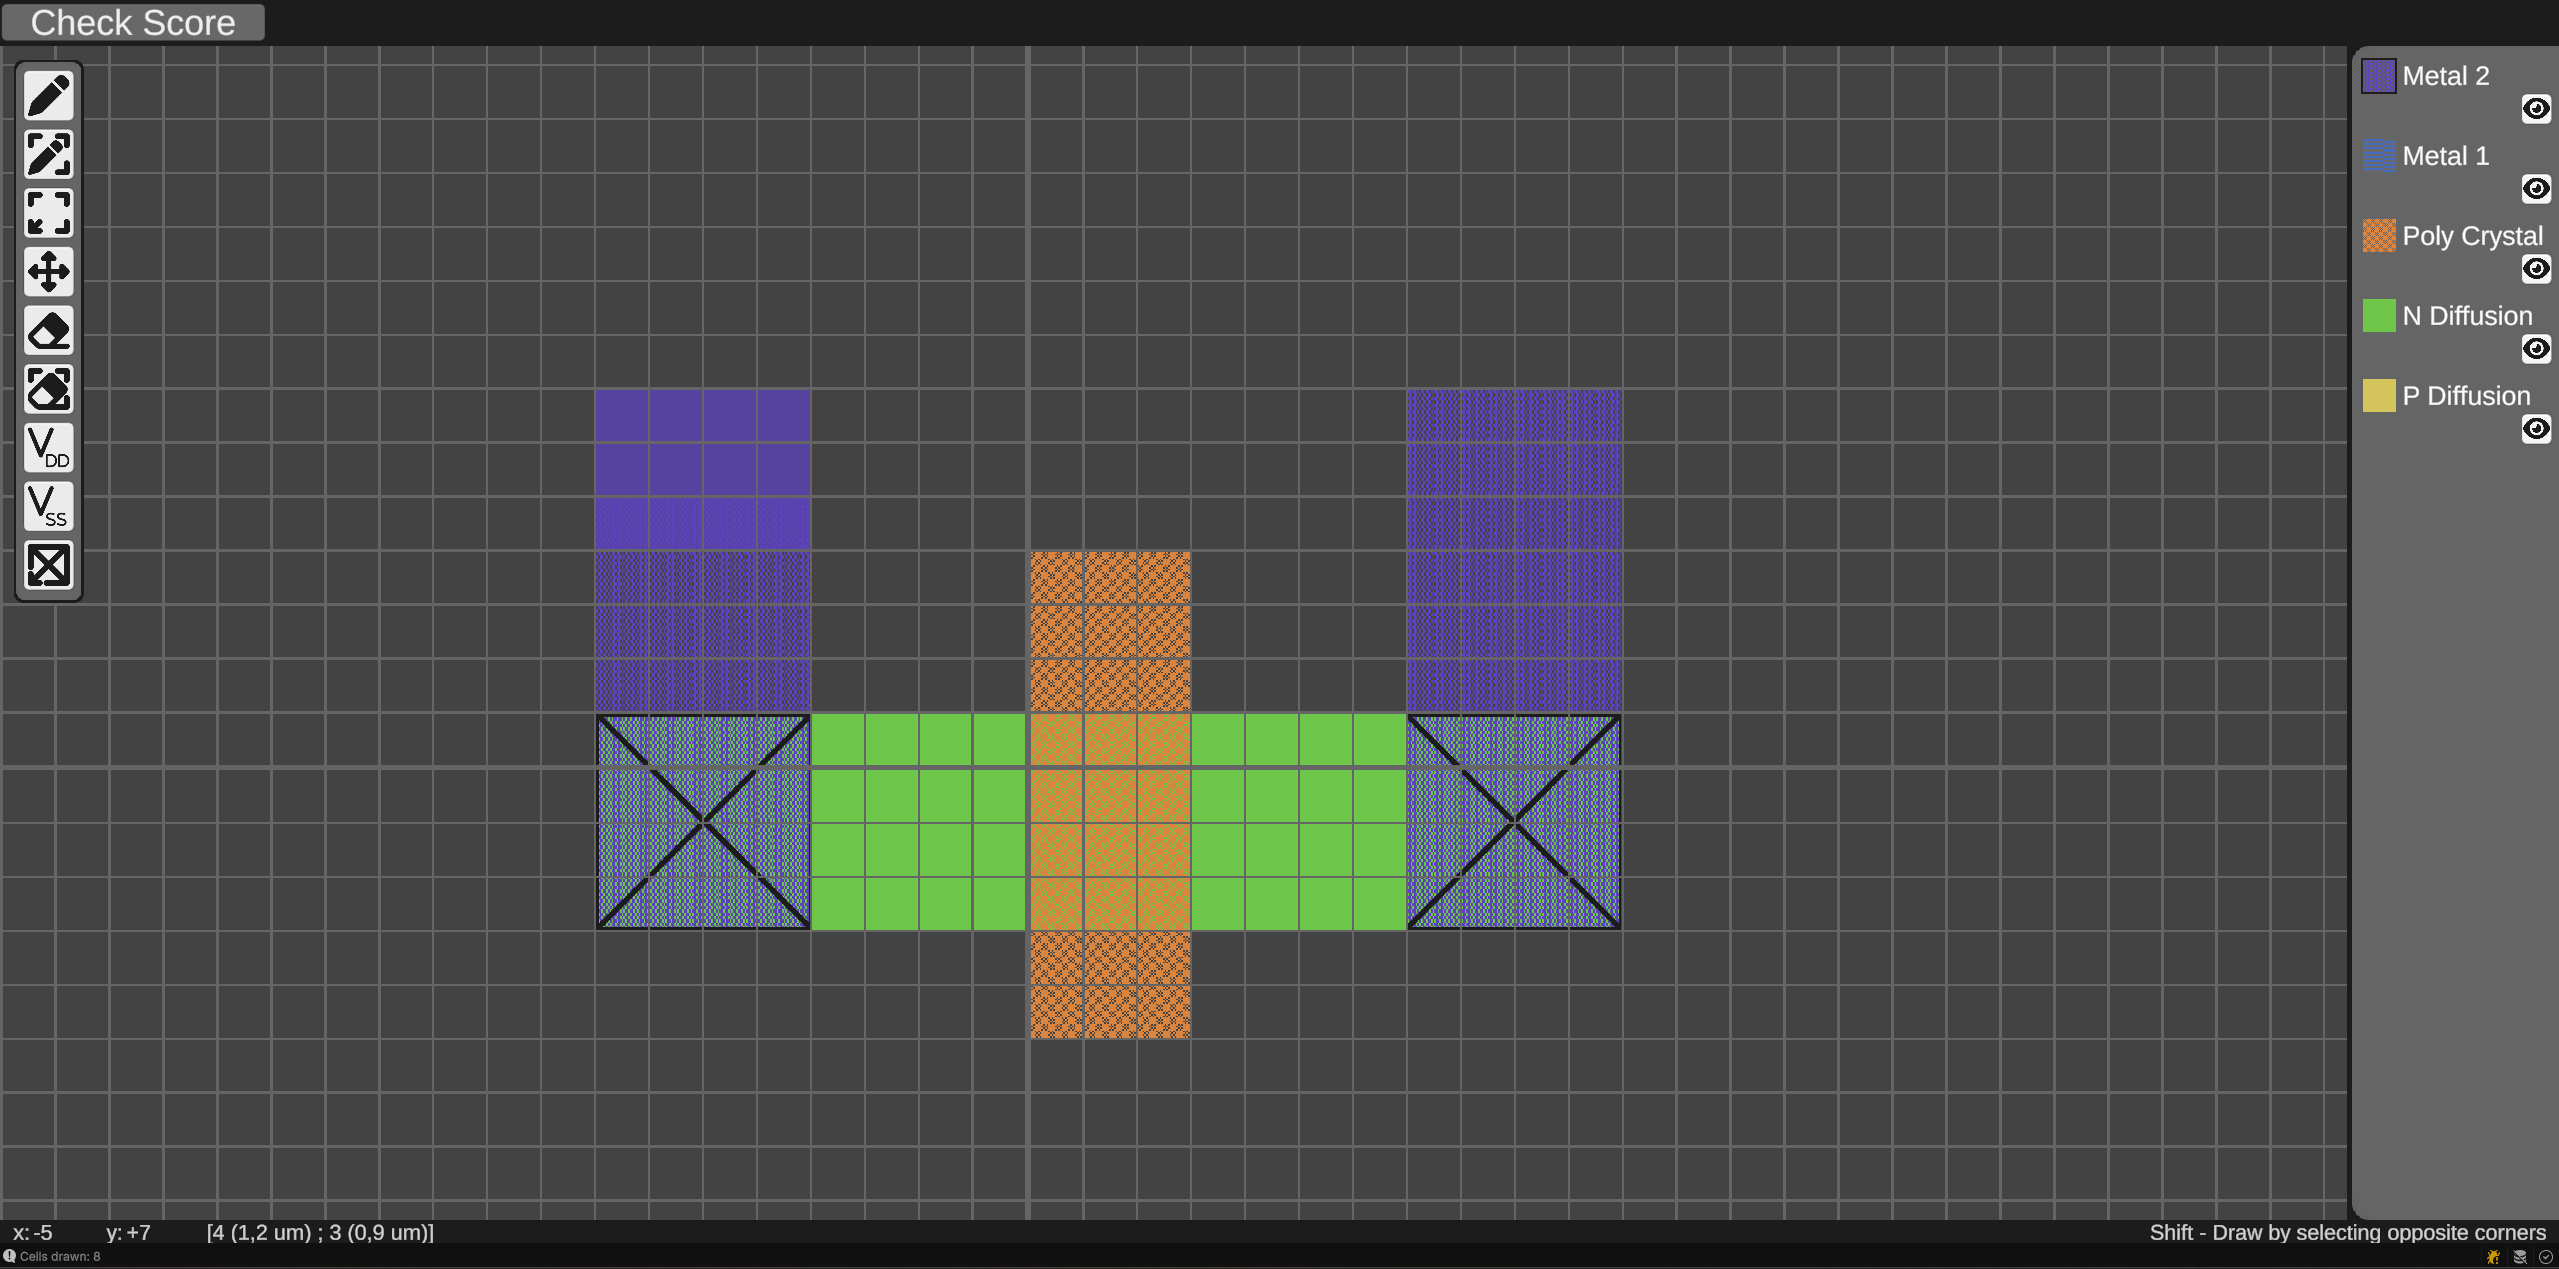
\includegraphics[width=0.9\textwidth]{chapters/chapter4/rys/final_ui}
    \caption[Widok okna aplikacji podczas pracy.]
    {Widok okna aplikacji podczas pracy, źródło: opracowanie własne.}
    \label{fig:ui_final}
\end{figure}

Z~prawej strony znajduje się panel warstw, który umożliwia wybór warstwy, którą użytkownik chce rysować.
Każda z~nich jest reprezentowana przez przycisk, który pozwala na jej wybór,
jej nazwę oraz dodatkowy przycisk do wyłączenia widoczności warstwy.
Panel taki dla każdej z~warstw jest generowany dynamicznie na podstawie konfiguracji warstw \texttt{LayerConfig},
pobrany z~menedżera warstw, \texttt{LayersManager}.
Na tej podstawie ustawiana jest nazwa warstwy oraz tekstura i~kolor w~przycisku wyboru.\\
%\indent Panel narzędzi znajduje się po lewej stronie okna.
%W~przeciwieństwie do warstw, przyciski do wyboru narzędzia są konfigurowane w~edytorze Unity,
%poprzez przypisanie im \texttt{ToolConfig}.
%To z~niego pobierane są informacje o ikonie narzędzia, podpowiedzi, jaka się wyświetli po najechaniu na przycisk
%oraz przypisany do narzędzi klawisz skrótu.\\
Panel narzędzi znajduje się po lewej stronie okna.
W~przeciwieństwie do warstw, przyciski wyboru narzędzia konfiguruje się w~edytorze Unity,
przypisując im \texttt{ToolConfig}.
Z~niego pobierane są informacje o ikonie,
podpowiedzi wyświetlanej po najechaniu na przycisk oraz przypisanym klawiszu skrótu.\\
\indent W~dolnej części okna znajduje się pasek informacyjny.
%Znajduje się tam wskaźnik aktualnej pozycji kursora na siatce, a~także dodatkowe informacje o narzędziu,
%takie jak klawisze modyfikujące działanie oraz komunikaty, jakie może te narzędzie przekazywać.
%Gdy wybrane jest narzędzie obszarowe,
%wyświetlana są dodatkowo wymiary zaznaczonego obszaru na siatce oraz wymiary przemnożone przez parametr $\lambda$.
%W~przypadku korzystania z~narzędzia przesuwania podawane są informacje o przemieszczeniu w~osiach $x$ i~$y$.
Panel zawiera wskaźnik aktualnej pozycji kursora na siatce oraz dodatkowe informacje o narzędziu,
takie jak klawisze modyfikujące jego działanie i~przekazywane przez niego komunikaty.
W~przypadku wybrania narzędzia obszarowego wyświetlane są wymiary zaznaczonego obszaru na siatce
oraz ich wartości przeliczone z~uwzględnieniem parametru $\lambda$.
Przy korzystaniu z~narzędzia przesuwania podawane są natomiast informacje o przemieszczeniu w~osiach $x$ i~$y$.
